\documentclass[tikz,border=10pt]{standalone}
\usepackage{tikz}
\usetikzlibrary{calc}

\begin{document}
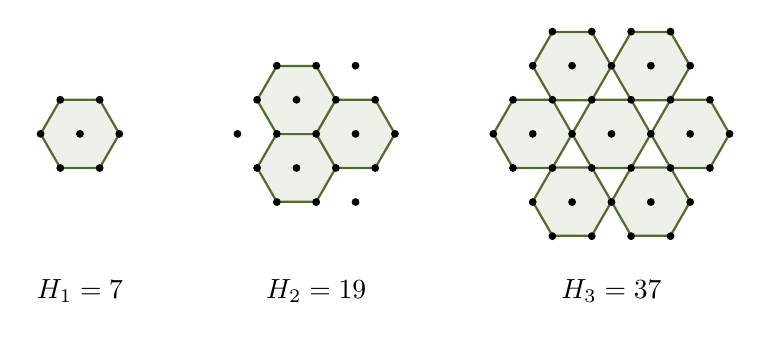
\begin{tikzpicture}[dot/.style={circle, fill=black, inner sep=1pt}]

%─────────────
% Controls
%─────────────
\def\hexstep{0.5}  % Distance from center to first ring point (controls scale)
\definecolor{olivegreen}{rgb}{0.33,0.42,0.18}  % Custom olive green

%───────────────────────────────────────────────────────
% Command to draw hexagons of side length 1
% Manually draw in hexagons for packing
%───────────────────────────────────────────────────────
\newcommand{\drawFirstRingHexagon}[3]{%
  \begin{scope}[shift={({#2},{#3})}]
    \foreach \i in {0,...,5} {
      \path (\i*60:#1) coordinate (P\i); % Place points every 60°
    }
    \filldraw[fill=olivegreen!10, draw=olivegreen, thick]
      (P0) -- (P1) -- (P2) -- (P3) -- (P4) -- (P5) -- cycle;
  \end{scope}
}

% H_1
\drawFirstRingHexagon{.5}{-3}{0}

% H_2
\drawFirstRingHexagon{.5}{-.25}{-.43}
\drawFirstRingHexagon{.5}{-.25}{.43}
\drawFirstRingHexagon{.5}{.5}{0}

% H_3
\drawFirstRingHexagon{.5}{3.75}{0}
\drawFirstRingHexagon{.5}{2.75}{0}
\drawFirstRingHexagon{.5}{4.75}{0}
\drawFirstRingHexagon{.5}{3.25}{.86}
\drawFirstRingHexagon{.5}{4.25}{.86}
\drawFirstRingHexagon{.5}{3.25}{-.86}
\drawFirstRingHexagon{.5}{4.25}{-.86}
% \drawFirstRingHexagon{.5}{3.75}{-.86}
% \drawFirstRingHexagon{.5}{3}{-.43}
% \drawFirstRingHexagon{.5}{3}{.43}
% \drawFirstRingHexagon{.5}{4.5}{-.43}
% \drawFirstRingHexagon{.5}{4.5}{.43}

%─────────────────────────────────────────────────────────────
% Draws a hexagonal lattice of dots:
% - #1 = number of rings (Hₙ)
% - (#2, #3) = x and y shift for placing center of structure
%─────────────────────────────────────────────────────────────
\newcommand{\drawHexagonDots}[3]{%
  \begin{scope}[shift={({#2},{#3})}]

    \pgfmathtruncatemacro{\rings}{#1}

    \ifnum\rings<1
      % If 0 or negative rings, do nothing
    \else
      % Always draw the central dot at the origin
      \node[dot] at (0,0) {};

      % Loop over each ring from 1 to total number
      \foreach \r in {1,...,\rings} {
        \pgfmathsetmacro{\rad}{\r * \hexstep}  % Radius for this ring

        % Each ring has 6 sides (hexagon)
        \foreach \side in {0,...,5} {
          \pgfmathsetmacro{\angleA}{60*\side}
          \pgfmathsetmacro{\angleB}{60*(\side+1)}

          % Define endpoints of one hex side arc at current radius
          \coordinate (A) at (\angleA:\rad);
          \coordinate (B) at (\angleB:\rad);

          % Interpolate points between A and B
          \foreach \k in {0,...,\numexpr\r-1} {
            \pgfmathsetmacro{\t}{\k/\r}
            \path ($(A)!{\t}!(B)$) node[dot] {};
          }
        }
      }
    \fi
  \end{scope}
}

%─────────────
% Draw examples H₁ through H₃
%─────────────
\drawHexagonDots{1}{-3}{0}     % H₁ = 7
\drawHexagonDots{2}{ 0}{0}     % H₂ = 19
\drawHexagonDots{3}{ 3.75}{0}  % H₃ = 37

%─────────────
% Labels
%─────────────
\node at (-3,-2) {$H_1 = 7$};
\node at ( 0,-2) {$H_2 = 19$};
\node at ( 3.75,-2) {$H_3 = 37$};

\end{tikzpicture}
\end{document}